\subsection{Dataset}
\label{app:dataset}

The data are split into train, validation and test. Every episode uses its
own world seed, and the seed ranges of the splits are disjoint (train from 0,
validation from 1M, test from 2M), so validation and test worlds are never
seen during training.

\emph{Train} (Table~\ref{tab:data-train}) has 2.0M frames (3\,529 episodes)
from a mix of the final PQN-RNN expert (70\% of the frames) and four earlier
snapshots of its training run (7.5\% each). Expert episodes are kept only if
they reach the diamond, and they end 500 steps after it, or earlier on death.
Snapshot episodes need no diamond and run until the agent dies.
\emph{Validation} (Table~\ref{tab:data-val}) has 151K frames (262 episodes)
and follows the same mix. \emph{Test} (Table~\ref{tab:data-test}) has 151K
frames (185 episodes) from the final expert only. It is the task set, used
only for planning and evaluation, never for training.

\begin{table}[H]
\centering
\caption{Composition and statistics of the training dataset by data-collection policy.}
\label{tab:data-train}
\small
\setlength{\tabcolsep}{3.5pt}
\begin{tabular}{lrrrrrrrr}
\toprule
Policy & Train steps & Share & Episodes & Length & Diamond & Return & Achiev. & Death \\
\midrule
Snapshot 1 & 50M & 7.5\% & 759 & 198 & 0.0\% & 6.83 & 7.73 & 100\% \\
Snapshot 2 & 150M & 7.5\% & 400 & 375 & 0.0\% & 16.08 & 16.98 & 100\% \\
Snapshot 3 & 300M & 7.5\% & 327 & 459 & 0.0\% & 16.85 & 17.75 & 100\% \\
Snapshot 4 & 400M & 7.5\% & 293 & 513 & 0.3\% & 17.79 & 18.69 & 100\% \\
Final expert & 1000M & 70.0\% & 1\,750 & 800 & 100.0\% & 20.60 & 21.10 & 46.7\% \\
\midrule
All & --- & 100\% & 3\,529 & 567 & 49.6\% & 16.54 & 17.24 & 73.6\% \\
\bottomrule
\end{tabular}

\vspace{4pt}
\begin{minipage}{\linewidth}
\footnotesize\raggedright
\textbf{Columns.} Policy: the policy that collected the episodes. Train steps: environment steps of PQN-RNN training at which the snapshot was taken. Share: fraction of frames. Episodes: number of episodes. Length: mean frames per episode. Diamond: fraction of episodes that collect a diamond. Return: mean undiscounted episode return. Achiev.: mean number of distinct achievements (of 22) unlocked per episode. Death: fraction of episodes that end in death; the remaining expert episodes end 500 steps after the diamond.
\end{minipage}
\end{table}

\begin{table}[H]
\centering
\caption{Composition and statistics of the validation dataset by data-collection policy.}
\label{tab:data-val}
\small
\setlength{\tabcolsep}{3.5pt}
\begin{tabular}{lrrrrrrrr}
\toprule
Policy & Train steps & Share & Episodes & Length & Diamond & Return & Achiev. & Death \\
\midrule
Snapshot 1 & 50M & 7.5\% & 56 & 202 & 0.0\% & 6.96 & 7.86 & 100\% \\
Snapshot 2 & 150M & 7.5\% & 31 & 363 & 0.0\% & 16.07 & 16.97 & 100\% \\
Snapshot 3 & 300M & 7.8\% & 23 & 513 & 0.0\% & 16.88 & 17.78 & 100\% \\
Snapshot 4 & 400M & 7.5\% & 24 & 471 & 0.0\% & 17.85 & 18.75 & 100\% \\
Final expert & 1000M & 69.7\% & 128 & 823 & 100.0\% & 20.65 & 21.15 & 46.1\% \\
\midrule
All & --- & 100\% & 262 & 576 & 48.9\% & 16.60 & 17.30 & 73.7\% \\
\bottomrule
\end{tabular}

\vspace{4pt}
\begin{minipage}{\linewidth}
\footnotesize\raggedright
\textbf{Columns.} Policy: the policy that collected the episodes. Train steps: environment steps of PQN-RNN training at which the snapshot was taken. Share: fraction of frames. Episodes: number of episodes. Length: mean frames per episode. Diamond: fraction of episodes that collect a diamond. Return: mean undiscounted episode return. Achiev.: mean number of distinct achievements (of 22) unlocked per episode. Death: fraction of episodes that end in death; the remaining expert episodes end 500 steps after the diamond.
\end{minipage}
\end{table}

\begin{table}[H]
\centering
\caption{Statistics of the test dataset, collected with the final expert only.}
\label{tab:data-test}
\small
\setlength{\tabcolsep}{3.5pt}
\begin{tabular}{lrrrrrrrr}
\toprule
Policy & Train steps & Share & Episodes & Length & Diamond & Return & Achiev. & Death \\
\midrule
Final expert & 1000M & 100\% & 185 & 814 & 100.0\% & 20.55 & 21.10 & 51.9\% \\
\bottomrule
\end{tabular}

\vspace{4pt}
\begin{minipage}{\linewidth}
\footnotesize\raggedright
\textbf{Columns.} Policy: the policy that collected the episodes. Train steps: environment steps of PQN-RNN training at which the policy was taken. Share: fraction of frames. Episodes: number of episodes. Length: mean frames per episode. Diamond: fraction of episodes that collect a diamond. Return: mean undiscounted episode return. Achiev.: mean number of distinct achievements (of 22) unlocked per episode. Death: fraction of episodes that end in death; the remaining episodes end 500 steps after the diamond.
\end{minipage}
\end{table}

\begin{figure}[H]
\centering
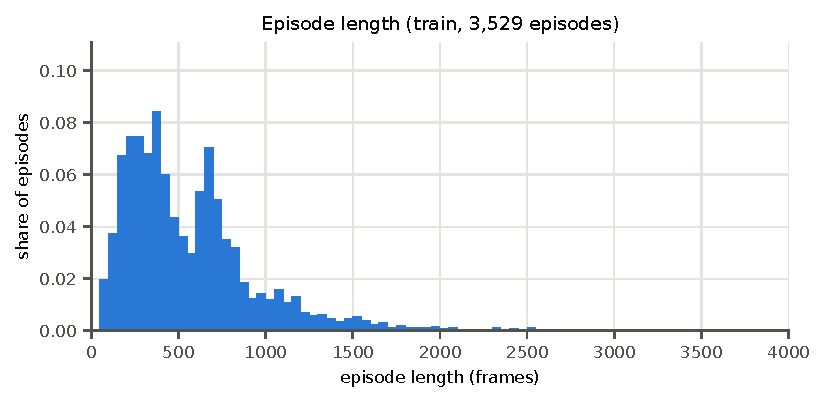
\includegraphics[width=\linewidth]{fig_length_train.pdf}
\caption{Episode length in the training split (bins of 50 frames). The test figure uses the same axes.}
\label{fig:data-length-train}
\end{figure}

\begin{figure}[H]
\centering
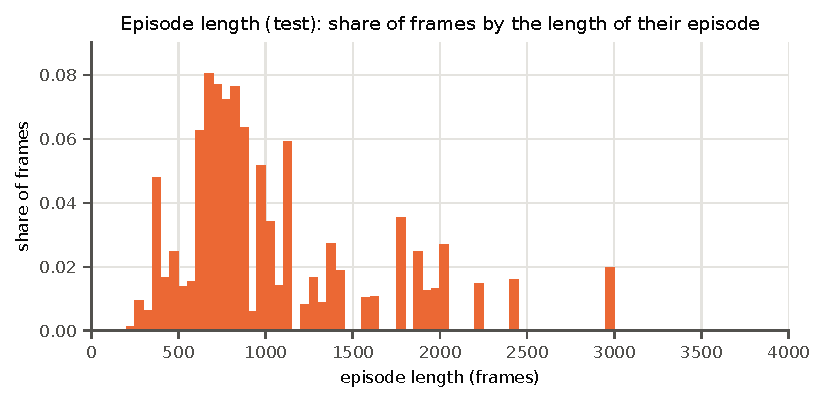
\includegraphics[width=\linewidth]{fig_length_test.pdf}
\caption{Episode length in the test split (bins of 50 frames), on the same axes as the training split.}
\label{fig:data-length-test}
\end{figure}

\begin{table}[H]
\centering
\caption{Episode length and time to the diamond, in frames.}
\label{tab:data-length}
\small
\setlength{\tabcolsep}{3.5pt}
\begin{tabular}{lrrrrrrrrr}
\toprule
& $n$ & Mean & Min & p10 & p25 & Median & p75 & p90 & Max \\
\midrule
Train, episode length & 3\,529 & 567 & 35 & 183 & 286 & 464 & 725 & 1\,072 & 3\,933 \\
Test, episode length & 185 & 814 & 201 & 384 & 554 & 729 & 916 & 1\,351 & 2\,987 \\
\midrule
Test, time to diamond & 185 & 476 & 99 & 148 & 199 & 313 & 594 & 922 & 2\,638 \\
\bottomrule
\end{tabular}

\vspace{4pt}
\begin{minipage}{\linewidth}
\footnotesize\raggedright Time to diamond: steps from the reset to the first frame with the diamond, over the episodes that reach it. Episodes that reach the diamond end 500 steps after it (or earlier on death).
\end{minipage}
\end{table}

\begin{figure}[H]
\centering
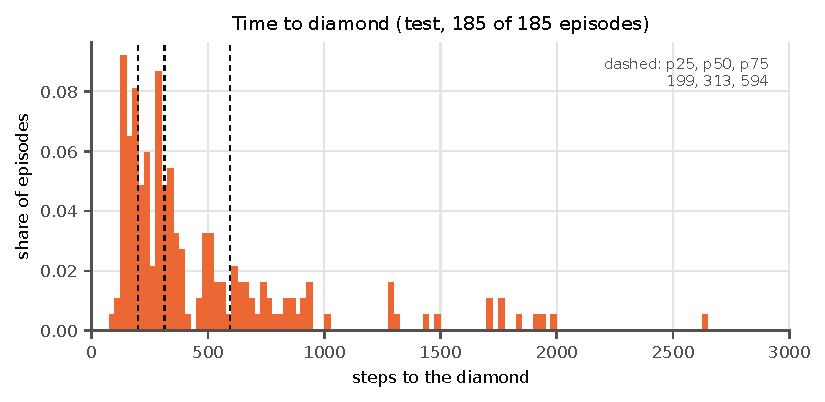
\includegraphics[width=\linewidth]{fig_time_to_diamond.pdf}
\caption{Steps from the reset to the first diamond in the test split (bins of 25 steps). Dashed lines: 25th, 50th and 75th percentile.}
\label{fig:data-time-to-diamond}
\end{figure}

\begin{table}[H]
\centering
\caption{Spectral centroid period of the probe entities of the test split.}
\label{tab:data-spectral}
\small
\setlength{\tabcolsep}{3.5pt}
\begin{tabular}{llrl}
\toprule
Entity & Group & Period & Limited \\
\midrule
facing & fast & 9.5 & no \\
mobs in view & fast & 15.8 & no \\
inventory & slow & 41.4 & yes \\
vitals & medium & 69.3 & yes \\
achievements & slow & 77.6 & yes \\
position & fast & 143.4 & yes \\
daylight & slow & 217.6 & yes \\
\bottomrule
\end{tabular}

\vspace{4pt}
\begin{minipage}{\linewidth}
\footnotesize\raggedright Centroid period in frames (1 / spectral centroid, Welch window 256, hop 128, Hann; each dimension standardised per episode), 184 test episodes. Limited: more than half of the power in the two lowest bins, so the period is a lower bound. Frequency gap (largest over smallest period): 23 or more, bootstrap p5 to p95 22.7 to 23.4; at windows 64: 8.32, 128: 14, 256: 23, 512: 28.6.
\end{minipage}
\end{table}

\begin{figure}[H]
\centering
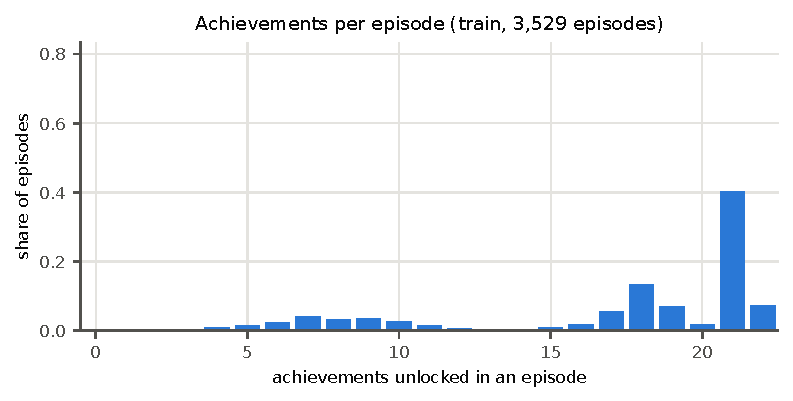
\includegraphics[width=\linewidth]{fig_achievements_train.pdf}
\caption{Distinct achievements (of 22) unlocked per episode in the training split.}
\label{fig:data-achievements-train}
\end{figure}

\begin{figure}[H]
\centering
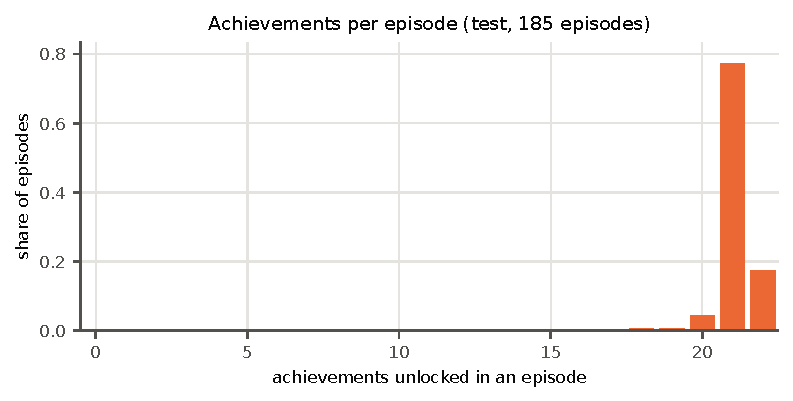
\includegraphics[width=\linewidth]{fig_achievements_test.pdf}
\caption{Distinct achievements (of 22) unlocked per episode in the test split, on the same axes as the training split.}
\label{fig:data-achievements-test}
\end{figure}

\begin{figure}[H]
\centering
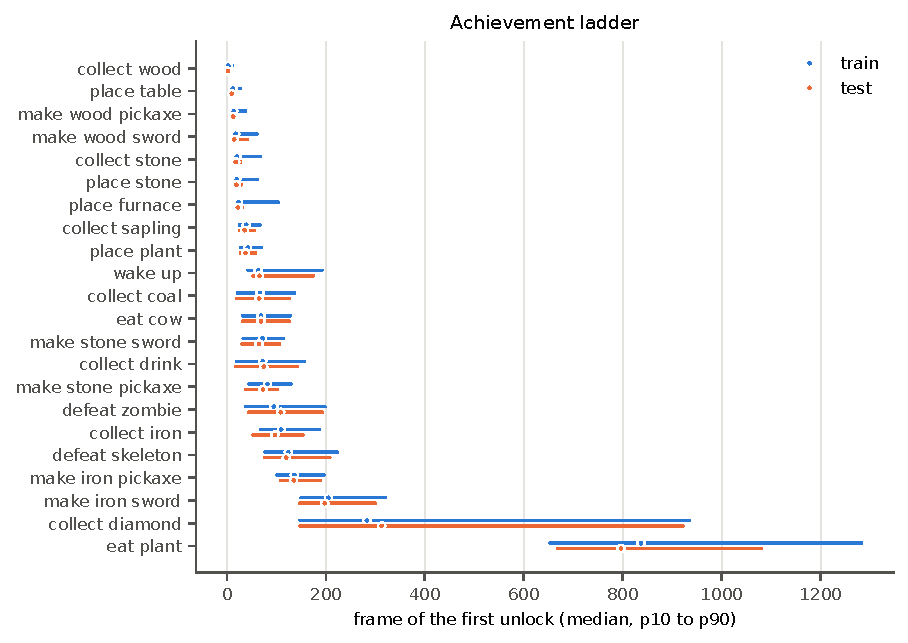
\includegraphics[width=\linewidth]{fig_achievement_ladder.pdf}
\caption{Frame of the first unlock of each achievement, over the episodes that unlock it: median and 10th to 90th percentile, sorted by the training median.}
\label{fig:data-ladder}
\end{figure}

\begin{table}[H]
\centering
\caption{Achievements: share of episodes that unlock each one and the frame of its first unlock.}
\label{tab:data-achievements}
\small
\setlength{\tabcolsep}{3.5pt}
\begin{tabular}{lrrrr}
\toprule
& \multicolumn{2}{c}{Train} & \multicolumn{2}{c}{Test} \\
 Achievement & Share & First unlock & Share & First unlock \\
\midrule
collect wood & 99.9\% & 3 [2, 11] & 100.0\% & 2 [2, 4] \\
place table & 99.5\% & 12 [8, 27] & 100.0\% & 10 [7, 16] \\
make wood pickaxe & 95.4\% & 14 [10, 38] & 100.0\% & 13 [10, 18] \\
make wood sword & 87.6\% & 18 [11, 61] & 100.0\% & 15 [10, 41] \\
collect stone & 91.9\% & 20 [14, 68] & 100.0\% & 18 [13, 28] \\
place stone & 88.9\% & 20 [15, 61] & 100.0\% & 19 [14, 29] \\
place furnace & 90.7\% & 23 [17, 104] & 100.0\% & 22 [16, 32] \\
collect sapling & 90.5\% & 39 [25, 67] & 99.5\% & 36 [26, 56] \\
place plant & 89.5\% & 42 [28, 69] & 99.5\% & 38 [27, 58] \\
wake up & 95.9\% & 63 [43, 192] & 98.9\% & 66 [53, 174] \\
collect coal & 79.0\% & 67 [21, 137] & 100.0\% & 65 [19, 126] \\
eat cow & 85.6\% & 69 [32, 129] & 100.0\% & 69 [32, 127] \\
make stone sword & 77.9\% & 72 [33, 114] & 100.0\% & 65 [30, 107] \\
collect drink & 85.1\% & 72 [19, 157] & 99.5\% & 74 [18, 143] \\
make stone pickaxe & 77.8\% & 82 [45, 130] & 100.0\% & 73 [38, 102] \\
defeat zombie & 77.8\% & 95 [38, 198] & 100.0\% & 109 [44, 194] \\
collect iron & 74.4\% & 110 [69, 187] & 100.0\% & 97 [52, 154] \\
defeat skeleton & 74.7\% & 124 [77, 224] & 100.0\% & 120 [77, 208] \\
make iron pickaxe & 56.8\% & 136 [101, 196] & 100.0\% & 135 [108, 188] \\
make iron sword & 48.6\% & 205 [150, 320] & 95.7\% & 198 [147, 300] \\
collect diamond & 49.6\% & 283 [148, 935] & 100.0\% & 313 [148, 922] \\
eat plant & 7.4\% & 837 [653, 1283] & 17.3\% & 796 [668, 1080] \\
\bottomrule
\end{tabular}

\vspace{4pt}
\begin{minipage}{\linewidth}
\footnotesize\raggedright First unlock: median frame, with p10 and p90 in brackets, over the episodes that unlock it. Sorted by the train median.
\end{minipage}
\end{table}

\begin{figure}[H]
\centering
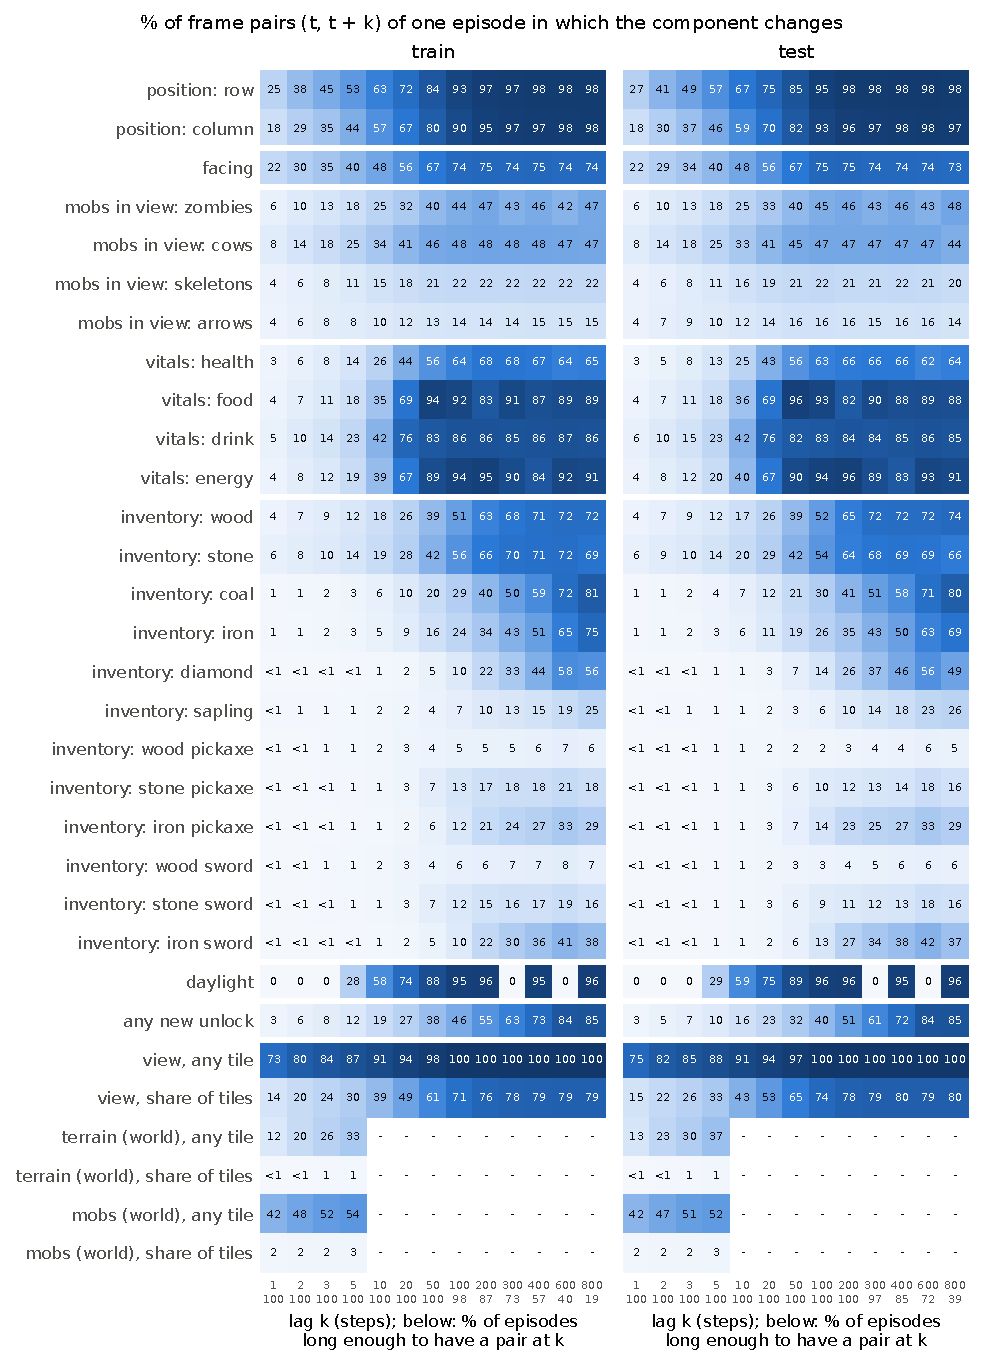
\includegraphics[width=\linewidth]{fig_change.pdf}
\caption{Share of frame pairs $(t, t+k)$ of one episode in which a state component has a different value, per lag $k$. The view rows are pooled over the 7$\times$9 tiles; the world-frame rows compare terrain and mobs in world coordinates on the tiles that both views show (lags up to 5). The second line of each tick is the percentage of episodes long enough to contain a pair at that lag. Daylight counts as changed above a difference of 0.05.}
\label{fig:data-change}
\end{figure}

\begin{figure}[H]
\centering
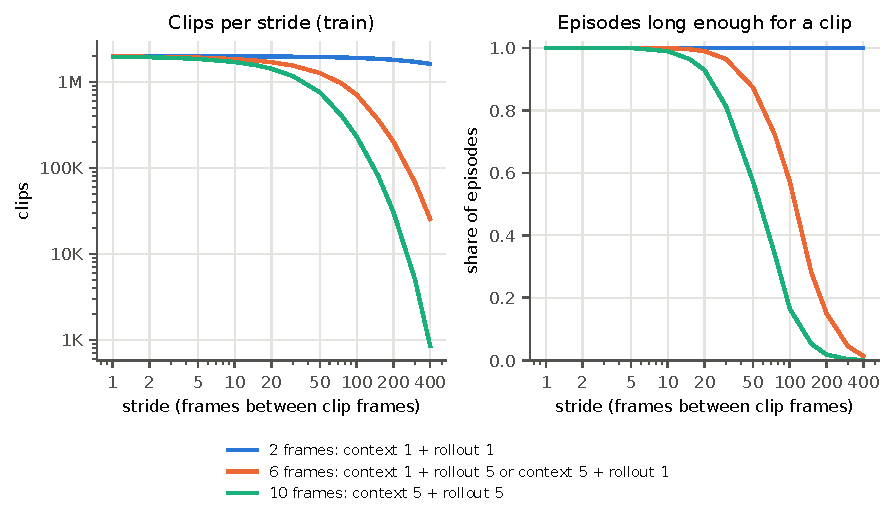
\includegraphics[width=\linewidth]{fig_clips.pdf}
\caption{Training clips per stride (all overlapping clips of the training split, with death padding as in training) and the share of episodes long enough to contain one, for clips of 2, 6 and 10 frames (context plus rollout).}
\label{fig:data-clips}
\end{figure}

\begin{figure}[H]
\centering
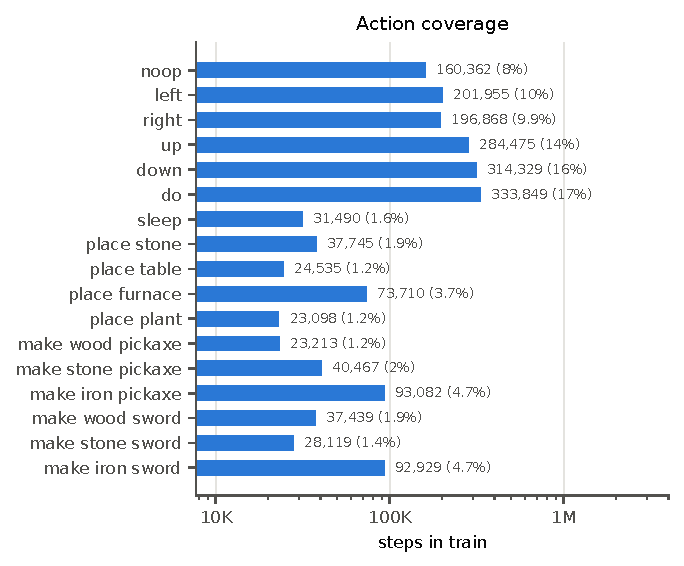
\includegraphics[width=\linewidth]{fig_actions.pdf}
\caption{Steps per action in the training split.}
\label{fig:data-actions}
\end{figure}

\begin{table}[H]
\centering
\caption{Action chunks of $k$ steps: distinct chunks, chunk entropy and information about the effect.}
\label{tab:data-chunks}
\small
\setlength{\tabcolsep}{3.5pt}
\begin{tabular}{lrrrrrrrr}
\toprule
& \multicolumn{4}{c}{Train} & \multicolumn{4}{c}{Test} \\
 $k$ & Distinct & $H$ & $I$ & Cov. & Distinct & $H$ & $I$ & Cov. \\
\midrule
1 & 17 & 3.5 & 1.94 & 100\% & 17 & 3.4 & 2.03 & 100\% \\
2 & 289 & 6.4 & 3.14 & 100\% & 284 & 6.2 & 3.33 & 99\% \\
3 & 4\,519 & 8.8 & 4.18 & 97\% & 2\,508 & 8.5 & 4.21 & 82\% \\
4 & 27\,550 & 10.9 & 4.88 & 82\% & 6\,958 & 10.3 & 4.90 & 59\% \\
6 & 102\,441 & 13.9 & 5.37 & 47\% & 13\,124 & 12.4 & 3.53 & 19\% \\
8 & 143\,096 & 15.5 & 4.11 & 22\% & 14\,240 & 13.1 & 1.88 & 9\% \\
12 & 139\,619 & 16.4 & 1.91 & 8\% & 11\,474 & 13.2 & 0.60 & 4\% \\
16 & 113\,645 & 16.4 & 0.99 & 5\% & 8\,954 & 13.0 & 0.61 & 3\% \\
\bottomrule
\end{tabular}

\vspace{4pt}
\begin{minipage}{\linewidth}
\footnotesize\raggedright Windows of $k$ steps without overlap (at most 500\,000 per $k$). Distinct: chunks seen. $H$: entropy of the chunk (bits). $I$: mutual information of the chunk with the effect (bits; change of inventory, achievements, vitals and position over the window; Miller--Madow corrected). Cov.: share of windows whose chunk was seen at least 20 times, the only windows $I$ is computed on; where it is low, most chunks occur once and $I$ is not reliable. Reference scales for a codebook, not settings.
\end{minipage}
\end{table}
